%% -*- coding: utf-8 -*-
\documentclass[12pt,a4paper]{scrartcl} 
\usepackage[utf8]{inputenc}
\usepackage[english,russian]{babel}
\usepackage{indentfirst}
\usepackage{misccorr}
\usepackage{graphicx}
\usepackage{amsmath}
\begin{document}
	\begin{titlepage}
		\begin{center}
			\large
			МИНИСТЕРСТВО НАУКИ И ВЫСШЕГО ОБРАЗОВАНИЯ РОССИЙСКОЙ ФЕДЕРАЦИИ
			
			Федеральное государственное бюджетное образовательное учреждение высшего образования
			
			\textbf{АДЫГЕЙСКИЙ ГОСУДАРСТВЕННЫЙ УНИВЕРСИТЕТ}
			\vspace{0.25cm}
			
			Инженерно-физический факультет
			
			Кафедра автоматизированных систем обработки информации и управления
			\vfill

			\vfill
			
			\textsc{Отчет по практике}\\[5mm]
			
			{\LARGE \textit{Найти определитель матрицы.}}
			\bigskip
			
			2 курс, группа 2ИВТ
		\end{center}
		\vfill
		
		\newlength{\ML}
		\settowidth{\ML}{«\underline{\hspace{0.7cm}}» \underline{\hspace{2cm}}}
		\hfill\begin{minipage}{0.5\textwidth}
			Выполнил:\\
			\underline{\hspace{\ML}} Н.\,А.~Свериденко\\
			«\underline{\hspace{0.7cm}}» \underline{\hspace{2cm}} 2021 г.
		\end{minipage}%
		\bigskip
		
		\hfill\begin{minipage}{0.5\textwidth}
			Руководитель:\\
			\underline{\hspace{\ML}} С.\,В.~Теплоухов\\
			«\underline{\hspace{0.7cm}}» \underline{\hspace{2cm}} 2021 г.
		\end{minipage}%
		\vfill
		
		\begin{center}
			Майкоп, 2021 г.
		\end{center}
	\end{titlepage}
	\section{Введение}
\label{sec:intro}

\begin{enumerate}
 \item Нужно написать программу, которая вычисляет определитель матрицы.
 \item Код программы, решающей задачу.
 \item Скриншот работы программы.
\end{enumerate}

\section{Ход работы}
\label{sec:exp}

\subsection{Код приложения}
\label{sec:exp:code}
\begin{verbatim}

#include <iostream>

class c_matrix
{
public:
    c_matrix(int a)
    {
        size = a;

        m = new float* [a];

        for (int i = 0; i < a; i++)
            m[i] = new float[a];
    };

    /* /void print()
    {
        for (int i = 0; i < size; i++)
        {
            for (int j = 0; j < size; j++)
            {
                std::cout << m[i][j] << " ";
            }

            std::cout << std::endl;
        }
    }; */

    c_matrix transponier()
    {
        c_matrix res(size);

        for (int i = 0; i < size; i++)
        {
            for (int j = 0; j < size; j++)
            {
                res.m[i][j] = m[i][j];
            }
        }

        float tmp;
        for (int k = 0; k < size - 1; k++) {
            for (int i = k + 1; i < size; i++) {
                tmp = -res.m[i][k] / res.m[k][k];
                for (int j = 0; j < size; j++) {
                    res.m[i][j] += res.m[k][j] * tmp;
                }
            }
        }

        return res;
    }

    float get_determinant()
    {
        c_matrix nn = transponier();

       // nn.print();

        float sum = 1;
        for (int i = 0; i < size; i++)
        {
            if (nn.m[i][i] != nn.m[i][i]) {
                sum = 0;
                break;
            }

            sum *= nn.m[i][i];
        }

        return sum;
    };

private:
    int size;
public:
    float** m;
};

int main()
{
    setlocale(LC_ALL, "RU");
    int size = 0;

    std::cout << "Enter matrix size: ";
    std::cin >> size;
    if (size <= 0)
    {
        std::cout << "Invalid matrix size." << std::endl;
        system("pause");
        return EXIT_FAILURE;
    }

    c_matrix m(size);

    std::cout << "Enter the matrix:" << std::endl;
    for (int i = 0; i < size; i++) {
        for (int j = 0; j < size; j++) {
            float in;
            std::cin >> in;

            if (std::cin.fail()) {
                std::cout << "Invalid value." << std::endl;

                system("pause");
                return EXIT_FAILURE;
            }
            else {
                m.m[i][j] = in;
            }
        }
    }

    std::cout << "Matrix determinant is: " << m.get_determinant() << "." << std::endl;

    system("pause");
    return EXIT_SUCCESS;
}
\end{verbatim}

\section{Скриншот программы}
\label{sec:picexample}
\begin{figure}[h]
	\centering
	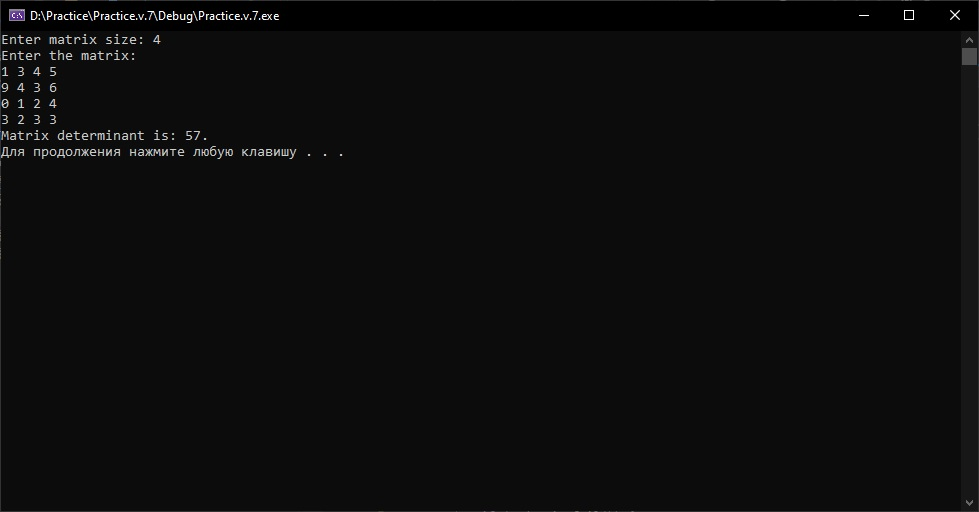
\includegraphics[width=0.8\textwidth]{practice.jpg}
	\caption{Работа программы}\label{fig:pra}
\end{figure}

Пример решения задачи представлен на рис.~\ref{fig:pra}.

\begin{thebibliography}{9}
\bibitem{Chakon}С. Чакон, Б. Штрауб. Git для профессионального программиста. \newblock --- Санкт-Петербург, 2016 г.
\bibitem{Lvovsky-2003}Львовский С.М. Набор и верстка в системе \LaTeX{}. \newblock --- 3-е издание, исправленное и дополненное, 2003 г.
\bibitem{Voroncov-2005}Воронцов К.В. \LaTeX{} в примерах. 2005 г.
\end{thebibliography}

\end{document}
